\documentclass[border=10pt,12pt]{standalone} 
\usepackage{graphicx}
\usepackage{tikz}
\usepackage{xcolor}
\usetikzlibrary{arrows,automata,decorations,chains,fit,quotes,shapes,positioning,calc}


\begin{document}

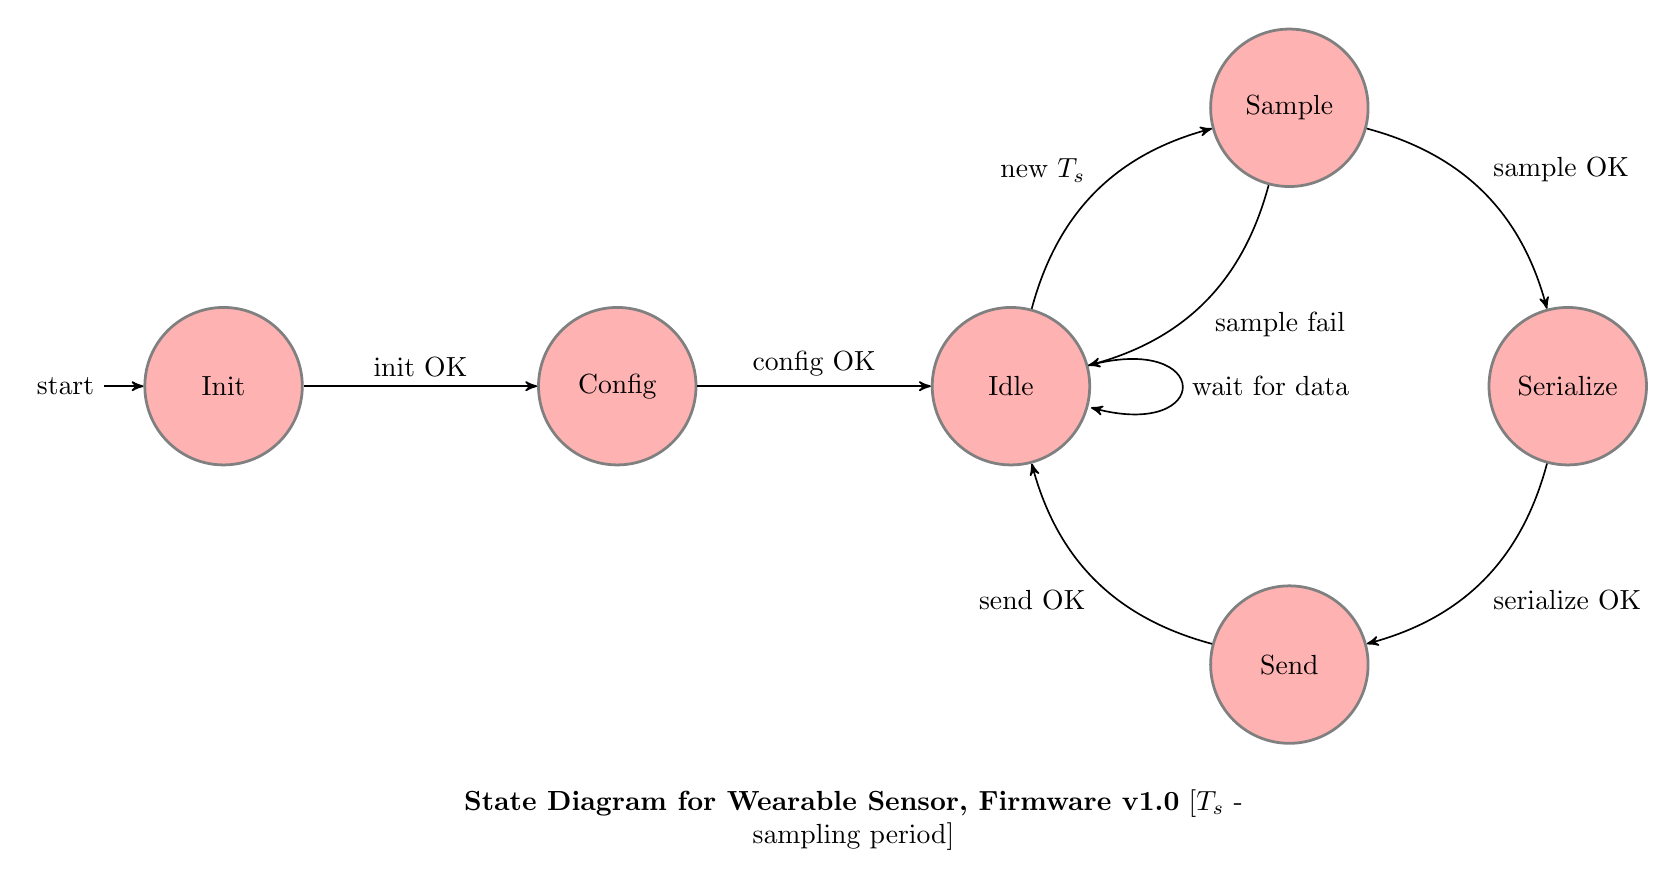
\begin{tikzpicture}[->,>=stealth',auto,node distance=5cm, semithick, transform shape, align=center,on grid,auto]

    \tikzstyle{every state}=[draw=gray,line width=1pt,circle,fill=red!30,text=black,minimum size=2cm]
    
    \node[initial, state, initial distance=.5cm] (A)    {Init};
    \node[state] (B) [right of = A]                     {Config};
    \node[state] (C) [right of = B]                     {Idle};
    \node[state] (D) [above right of = C]               {Sample};
    \node[state] (E) [below right of = D]               {Serialize};
    \node[state] (F) [below left of = E]                {Send};

    \path (A) edge              node                        {init OK}        (B)
          (B) edge              node                        {config OK}      (C)
          (C) edge [bend left]  node                        {new $T_s$}      (D)
              edge [loop right] node                        {wait for data}  (C)    
          (D) edge [bend left]  node                        {sample OK}      (E)
              edge [bend left]  node                        {sample fail}    (C)
          (E) edge [bend left]  node                        {serialize OK}   (F)
          (F) edge [bend left]  node                        {send OK}        (C);
    \node [below=6cm, align=flush center,text width=11cm] at (8,1) {\textbf{State Diagram for Wearable Sensor, Firmware v1.0} [$T_s$ - sampling period]};
\end{tikzpicture}
\end{document}